\section{Monte Carlo Tree Search (MCTS)}
\frame{\tableofcontents[currentsection, hideothersubsections]}

\begin{frame}
\frametitle{Monte Carlo Tree Search (MCTS)}
Based on 2 fundamental concepts:
\begin{itemize}
\item {\small the true value of an action may be approximated using random simulation}
\item these approximated values may be used efficiently to adjust the policy
\end{itemize}

\begin{figure}
    \centering
    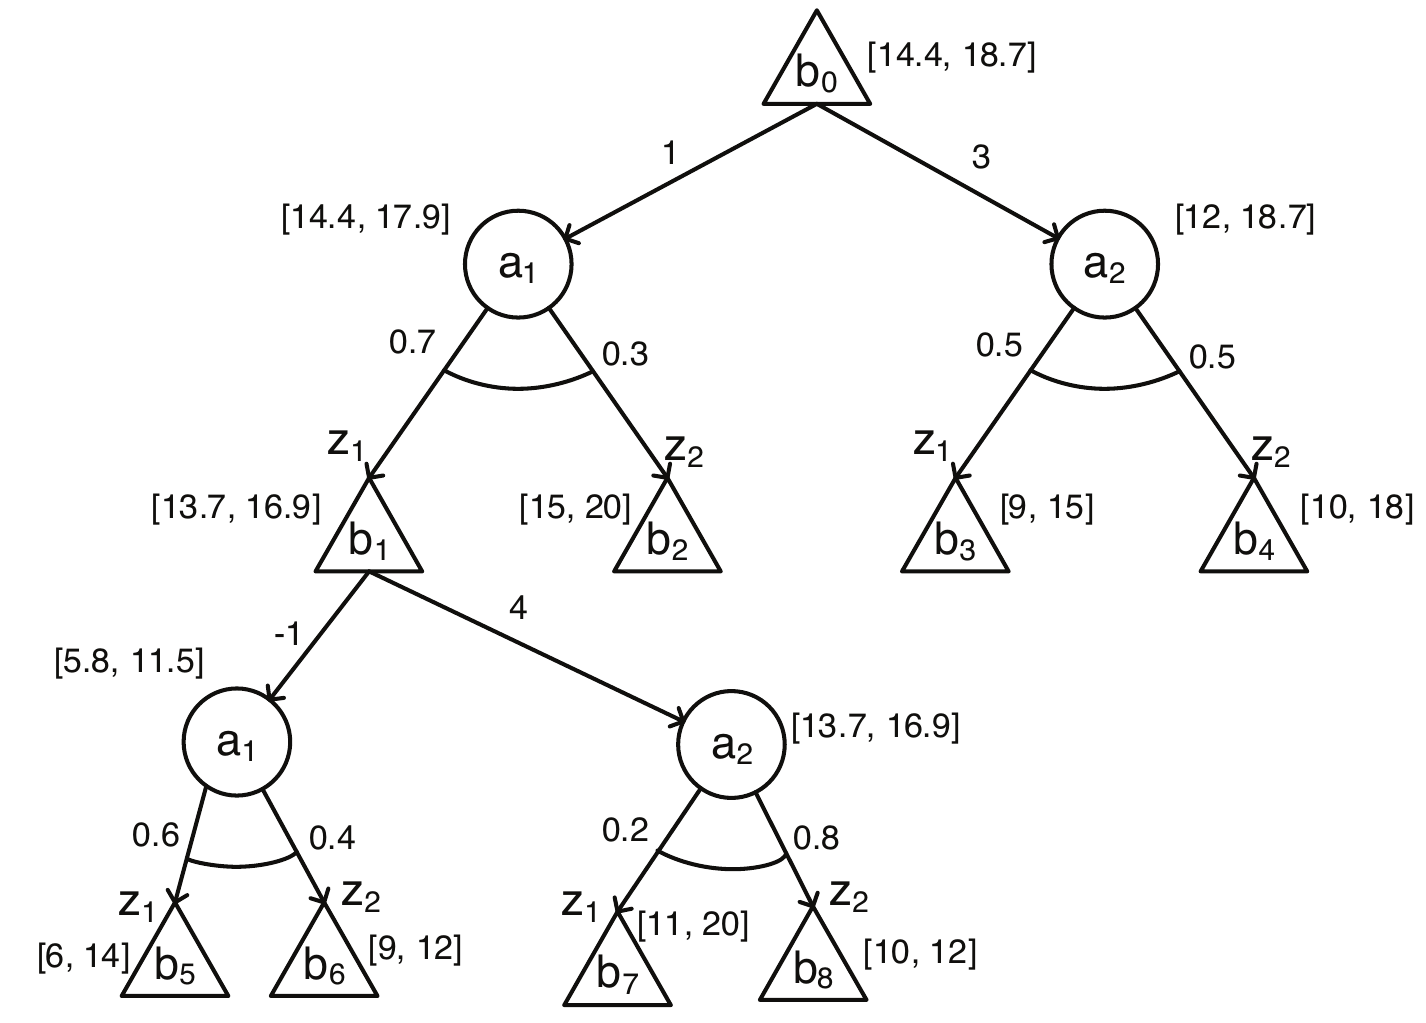
\includegraphics[scale=0.2]{and_or_tree}
\end{figure}

\end{frame}

\begin{frame}
\frametitle{Monte Carlo Tree Search (MCTS): Selection}
\begin{figure}
    \centering
    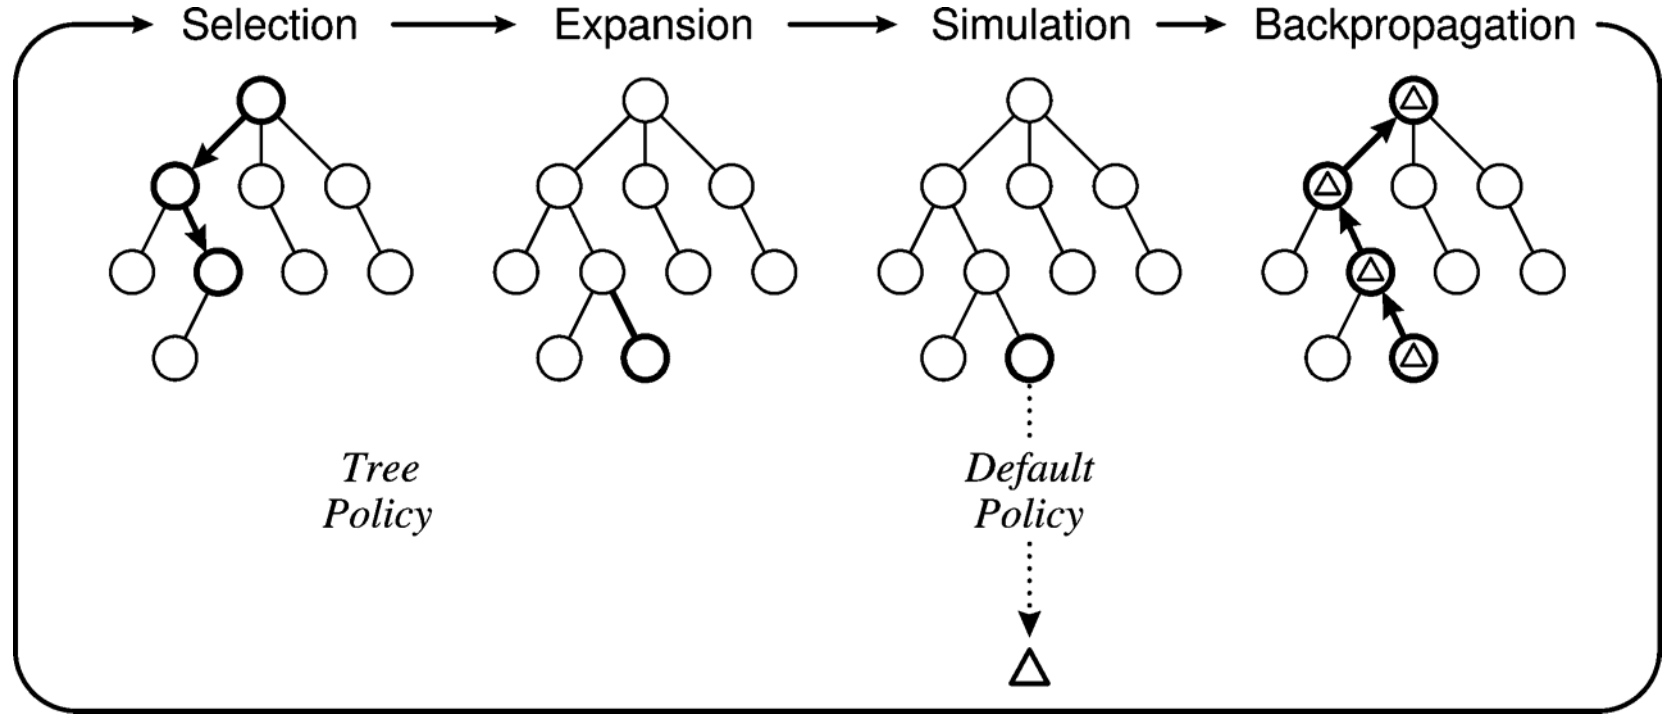
\includegraphics[scale=0.25]{mcts_steps}
\end{figure}

1) Selection:
\small
\begin{itemize}
\item starting at the root node, a child selection policy is recursively applied to descend through the tree until
the most urgent expandable node is reached
\item a node is expandable if it represents a nonterminal state and has unvisited (i.e., unexpanded) children.
\end{itemize}
\end{frame}

\begin{frame}
\frametitle{Monte Carlo Tree Search (MCTS): Expansion}
\begin{figure}
    \centering
    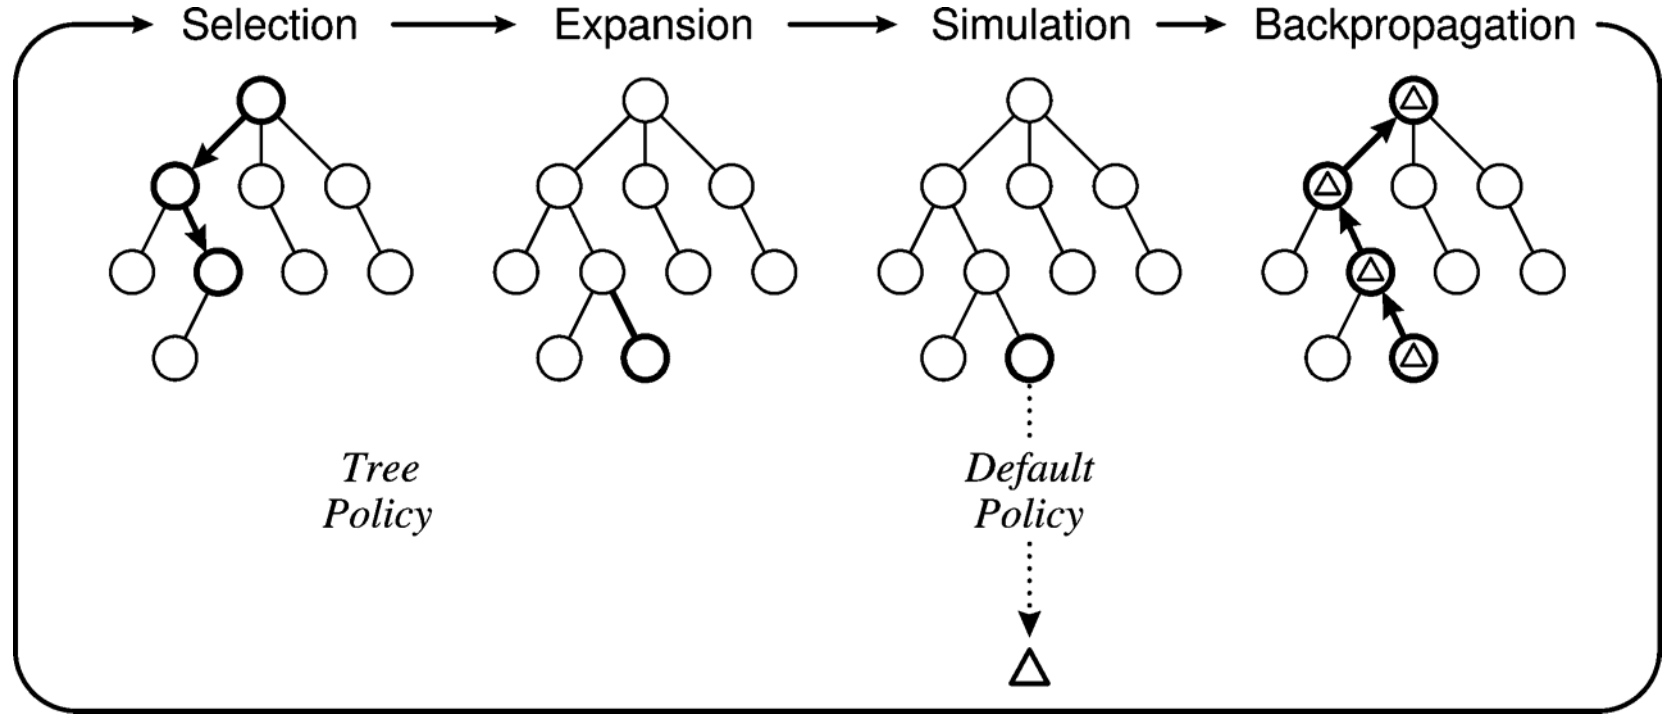
\includegraphics[scale=0.25]{mcts_steps}
\end{figure}

2) Expansion:
\small
\begin{itemize}
\item one (or more) child nodes are added to expand the tree, according to the available actions.
\end{itemize}
\end{frame}

\begin{frame}
\frametitle{Monte Carlo Tree Search (MCTS): Simulation}
\begin{figure}
    \centering
    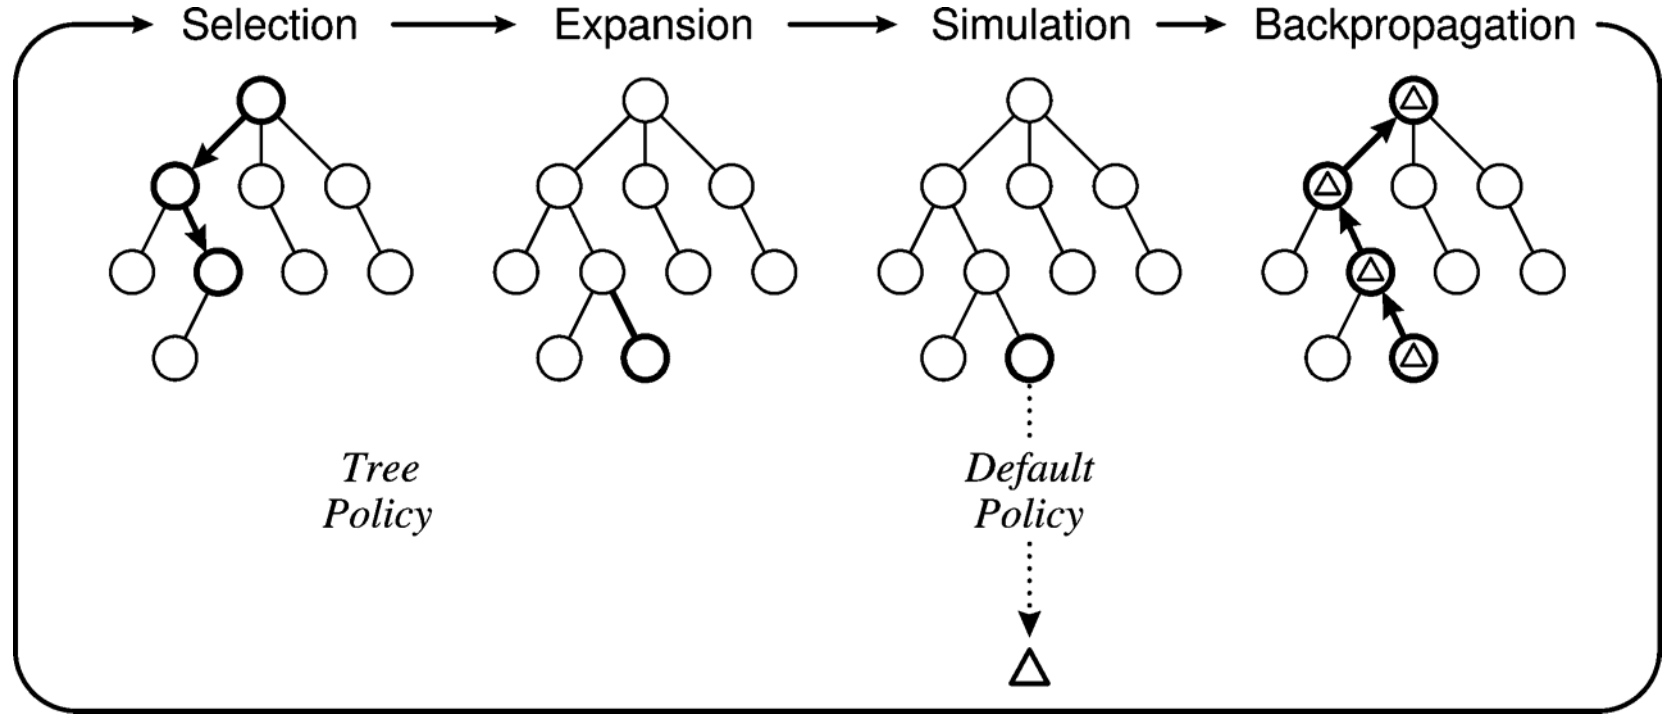
\includegraphics[scale=0.25]{mcts_steps}
\end{figure}

3) Simulation:
\small
\begin{itemize}
\item A simulation is run from the new node(s) according to the default policy to produce an outcome.
\end{itemize}
\end{frame}

\begin{frame}
\frametitle{Monte Carlo Tree Search (MCTS): Backpropagation}
\begin{figure}
    \centering
    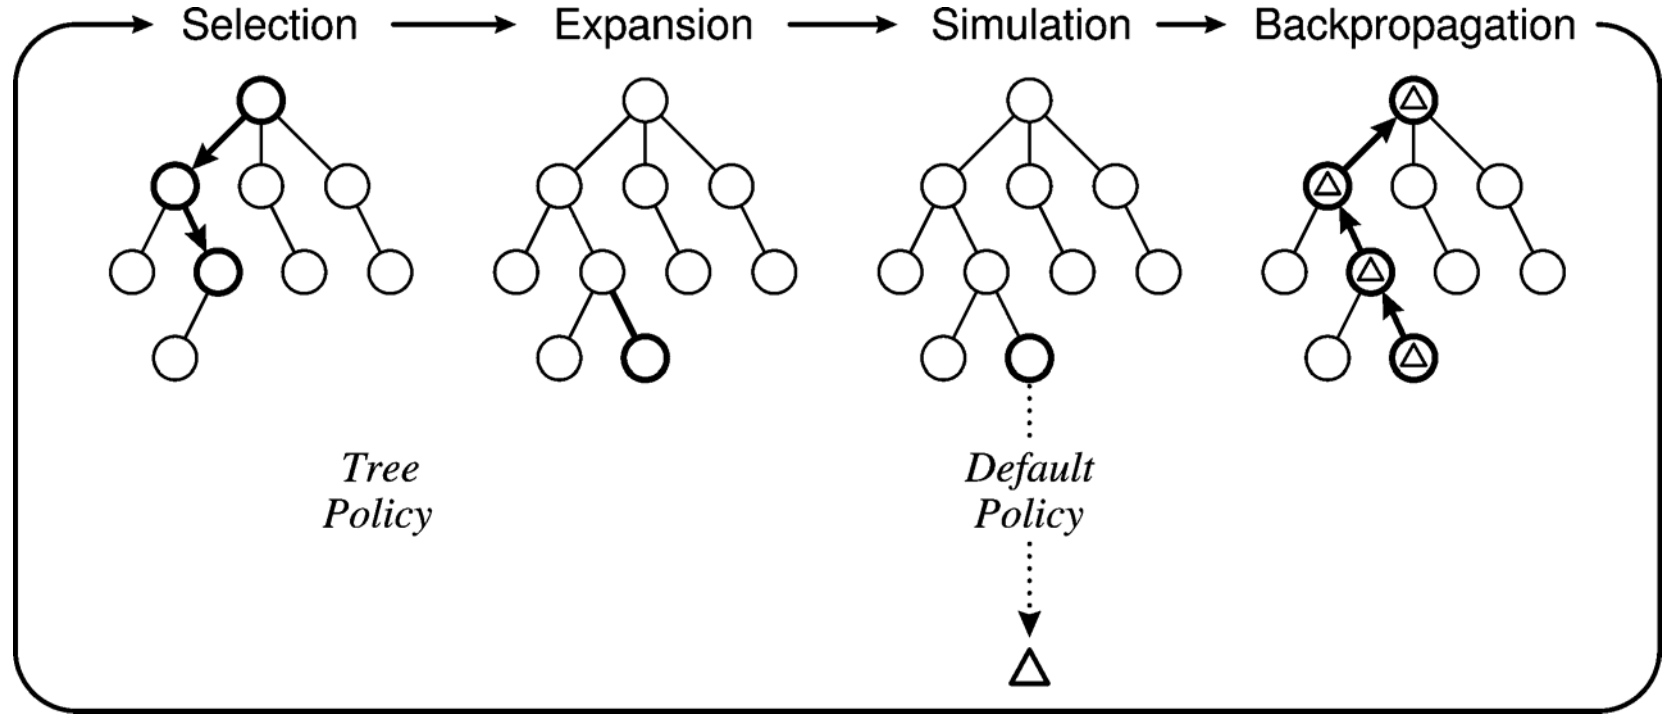
\includegraphics[scale=0.25]{mcts_steps}
\end{figure}

4) Backpropagation:
\small
\begin{itemize}
\item The simulation result is ``backed up'' (i.e., backpropagated) through the selected nodes to
update their statistics.
\end{itemize}
\end{frame}

\begin{frame}
\frametitle{Monte Carlo Tree Search (MCTS): UCT as tree policy}
UCT (UCB1 for Tree): \\
every time a node (action) is to be selected within the existing tree, \\
the choice may be modeled as an independent multiarmed bandit problem \\
\vspace{5mm}
\pause

A child node $j$ is selected to maximize:
\begin{equation*}
UCT = \bar{X}_j + 2 C_p \sqrt{\frac{2~ln~n}{n_j}}
\end{equation*}
\pause

\begin{itemize}
\item $\bar{X}_j$: the average reward from child node $j$ \pause
\item $n$: the number of times the current (parent) node has been visited, \pause
\item $n_j$: the number of times child node $j$ has been visited, \pause
\item $C_p > 0$: a constant.
\end{itemize}

\end{frame}